\section{Descrição de Hardware}

%\subsubsection{Objetivo do Hardware}

O objetivo principal do hardware é fornecer os meios eletrônicos e físicos para coletar os dados necessários para o controle de trajetória do foguete d'água e para automatizar o processo de lançamento. Isso envolve a integração de sensores para medir parâmetros como pressão, ângulo, altitude, velocidade e aceleração.

O hardware é projetado para trabalhar em conjunto com o software, onde os dados coletados pelos sensores são processados e utilizados para analisar trajetória do foguete. A escolha dos componentes de hardware é feita para garantir que eles atendam aos requisitos de desempenho do software, como a precisão das medições e a armazenar os dados.

%\textbf{Implementação do Hardware}

Para cumprir o objetivo de coletar dados de voo e controlar o sistema de lançamento, o hardware é implementado utilizando o microcontrolador ESP32 como o componente central de processamento. O desenvolvimento do código para o ESP32 será realizado na Arduino IDE (Integrated Development Environment), uma plataforma de desenvolvimento integrada que simplifica significativamente o processo de escrita, compilação, upload e depuração do código para microcontroladores. A escolha da Arduino IDE se deve à sua facilidade de uso, vasta comunidade de suporte e disponibilidade de bibliotecas, o que acelera o desenvolvimento e reduz a complexidade do projeto. A linguagem de programação utilizada será o "C", devido à sua eficiência, controle de baixo nível e adequação para sistemas embarcados onde o desempenho e o uso eficiente de recursos são críticos.

O microcontrolador ESP32 é responsável por orquestrar a coleta, o pré-processamento e o armazenamento dos dados provenientes do sensor. Para facilitar a interação com os diversos periféricos e garantir a modularidade e a reutilização do código, serão utilizadas bibliotecas específicas:

Para a comunicação com o módulo de cartão SD, será utilizada a biblioteca SD.h, que fornece um conjunto robusto de funções para leitura e escrita de dados em cartões SD no formato FAT32. Essa biblioteca permite a criação, abertura, leitura, escrita e fechamento de arquivos, bem como a manipulação de diretórios, garantindo a persistência dos dados de voo para análise posterior.

Para a leitura dos dados do sensor MPU-6500, será utilizada a biblioteca Adafruit MPU6050 (ou similar), que abstrai a complexidade da comunicação I2C com o sensor e fornece funções para a obtenção de dados de aceleração e velocidade angular em três eixos. Essa biblioteca simplifica a calibração do sensor e a conversão dos dados brutos em unidades físicas, facilitando o desenvolvimento do firmware.

O sensor MPU-6500, um componente essencial para a medição da orientação e do movimento do foguete, é instalado estrategicamente no foguete para capturar com precisão a aceleração e a velocidade angular durante o voo. Os dados coletados por este sensor são cruciais para a reconstrução da trajetória do foguete e para a análise do seu desempenho. Especificamente, o MPU-6500 fornece dados de aceleração linear nos três eixos cartesianos (x, y e z), permitindo determinar as forças que atuam sobre o foguete em cada direção, através da aplicação da segunda lei de Newton. A velocidade angular, também medida nos três eixos, é fundamental para compreender a rotação e a estabilidade do foguete durante o voo. A integração temporal dos dados de aceleração, combinada com a orientação obtida da velocidade angular, possibilita o cálculo do deslocamento do foguete ao longo do tempo, fornecendo informações detalhadas sobre a sua posição e trajetória no espaço. Simultaneamente, um módulo de leitura de cartão SD é integrado ao sistema para fornecer um meio de armazenamento local e não volátil para os dados de voo, atuando como um backup e garantindo que nenhum dado crítico se perca, mesmo em caso de falhas.

A arquitetura do firmware seguirá os princípios de sistemas de tempo real, priorizando a eficiência e o determinismo na execução das tarefas. O firmware será estruturado em um loop principal contínuo e determinístico, responsável pela execução cíclica das seguintes tarefas:

Leitura dos dados dos sensores: Os dados dos sensores, incluindo o MPU-6500, são amostrados periodicamente com uma frequência predefinida para garantir a captura adequada da dinâmica do voo.

Pré-processamento dos dados: Os dados brutos dos sensores podem ser filtrados ou convertidos em unidades físicas, se necessário, para reduzir o ruído e melhorar a precisão.

Detecção de eventos: O firmware monitora continuamente os dados dos sensores em busca de eventos significativos, como o início do lançamento, que podem ser detectados por variações bruscas na aceleração.

Armazenamento condicional dos dados: Os dados são armazenados no cartão SD apenas quando eventos significativos são detectados ou em intervalos regulares predefinidos, otimizando o uso do espaço de armazenamento e garantindo a preservação dos dados relevantes.

Essa abordagem de firmware em tempo real permite uma resposta rápida e eficiente aos eventos do voo, garantindo a coleta confiável dos dados e o controle preciso do sistema.


\usetikzlibrary{arrows.meta}
\usetikzlibrary{positioning}

\begin{figure}[h!]
    \centering
    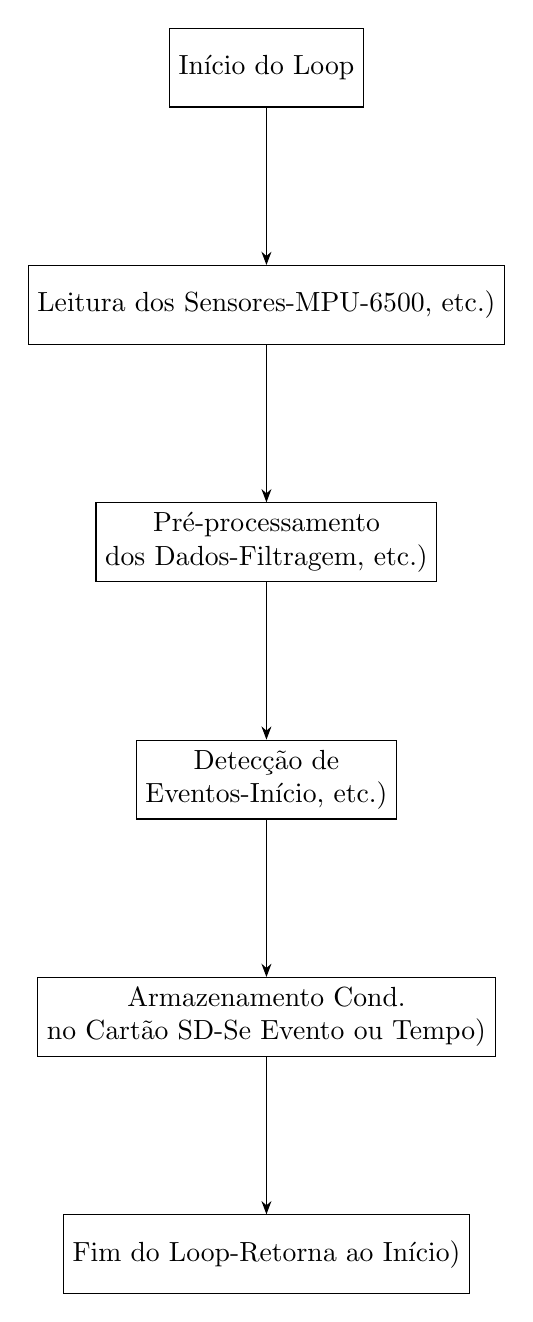
\begin{tikzpicture}[
        node distance=2cm,
        block/.style={rectangle, draw, minimum width=2cm, minimum height=1cm, align=center},
        cloud/.style={ellipse, draw, minimum width=2cm, minimum height=1cm, align=center},
        arrow/.style={-Stealth}  % UNCOMMENTED style definition
        ]

        % Nodes with modern positioning syntax
        \node (start)      [block] {Início do Loop};
        \node (read)       [block, below=of start] {Leitura dos Sensores-MPU-6500, etc.)};
        \node (preprocess) [block, below=of read]  {Pré-processamento\\dos Dados-Filtragem, etc.)};
        \node (detect)     [block, below=of preprocess] {Detecção de\\Eventos-Início, etc.)};
        \node (store)      [block, below=of detect]  {Armazenamento Cond.\\no Cartão SD-Se Evento ou Tempo)};
        \node (end)        [block, below=of store]   {Fim do Loop-Retorna ao Início)};

        % Arrows using the defined style
        \draw[arrow] (start)  -- (read);
        \draw[arrow] (read)       -- (preprocess);
        \draw[arrow] (preprocess) -- (detect);
        \draw[arrow] (detect)     -- (store);
        \draw[arrow] (store)      -- (end);
        %\draw[arrow] (end)        -- (start);

    \end{tikzpicture}
    \caption{Diagrama de Blocos do Firmware}
    \label{fig:firmware_diagram}
\end{figure}


\textbf{Seleção dos Componentes de Hardware}

A escolha dos componentes de hardware é baseada em objetivos específicos e na necessidade de criar um sistema coeso e eficiente.

\textbf{Microcontrolador ESP32:} Escolhido por sua capacidade de processamento e suporte para sensores e atuadores.

\textbf{Sensores (MPU-6500):} Selecionados por sua precisão e capacidade de fornecer dados confiáveis sobre o movimento do foguete.

\textbf{Módulo de cartão SD:} Selecionados por sua capacidade de armazenar dados coletados em um cartão SD, trazendo portabilidade ao sistema.

\textbf{Fonte de Energia:} Para energizar todo o sistema, será utilizada uma bateria LiPo de 1 célula (1S) com tensão de 4.2V. A alimentação será fornecida à entrada Vin de 3.3V do ESP32, que possui um regulador de tensão interno capaz de lidar com a tensão ligeiramente superior da bateria, garantindo a operação segura dos componentes.

Nesta etapa de seleção de componentes de hardware, estamos realizando uma abstração das complexidades inerentes ao fornecimento de energia para um sistema embarcado. Fatores como dimensionamento preciso da bateria, regulação de tensão para outros componentes, gerenciamento de carga/descarga, eficiência energética e dissipação de calor são considerações cruciais que impactam diretamente a estabilidade e a confiabilidade do sistema. No entanto, o detalhamento aprofundado dessas considerações, bem como a análise completa do sistema de energia, serão abordados na seção dedicada à "Energia" deste documento.

A combinação desses componentes permite a criação de um sistema de hardware robusto e eficiente, capaz de atender aos requisitos do projeto.


\begin{figure}[h!]
    \centering
    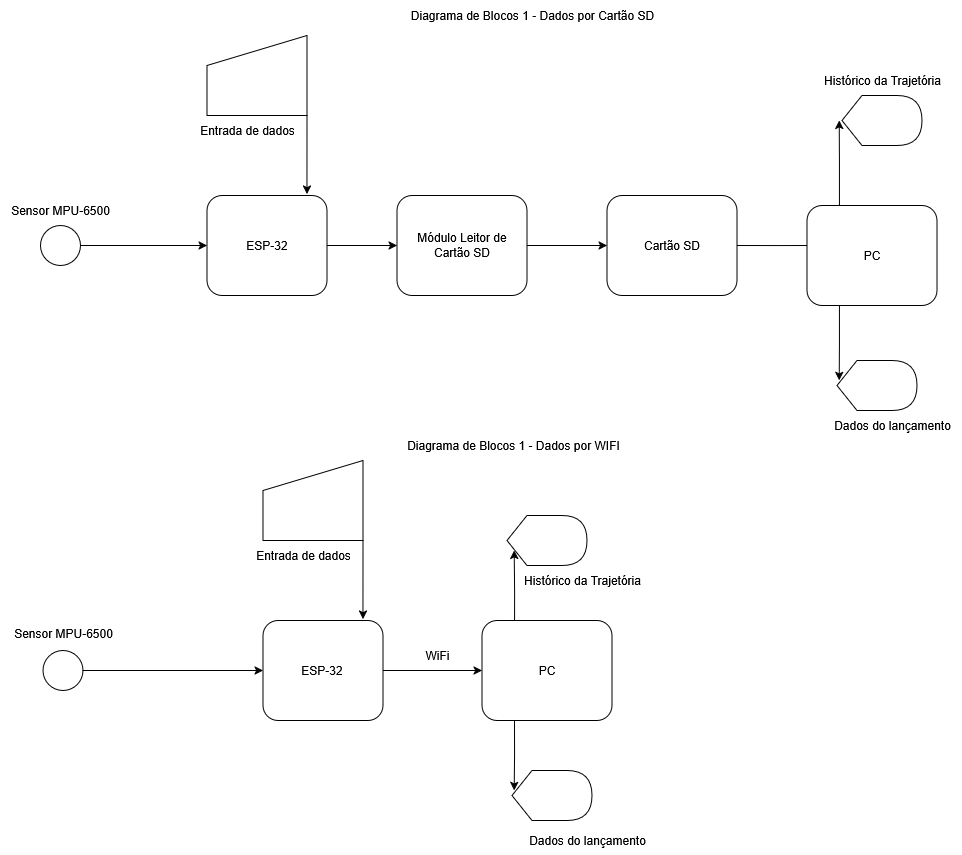
\includegraphics[width=0.8\textwidth]{figuras/diagramaDeBlocosHardware.png}

    \caption{Diagrama de Blocos do Hardware}
    \label{fig_diagrama_blocos_hardware}
\end{figure}

%\textbf{Esquemático de Conexões}

Esta seção detalha as conexões elétricas entre os componentes do sistema. É crucial observar que as informações fornecidas aqui são genéricas e podem variar dependendo dos modelos exatos dos componentes utilizados. Sempre consulte os datasheets dos componentes para obter informações precisas sobre os pinos e as especificações elétricas.

\paragraph{Representação Esquemática Básica}

A Figura \ref{fig:esquematico_basico} apresenta um diagrama esquemático simplificado das conexões entre os principais componentes do sistema.

\begin{figure}[H]
    \centering
    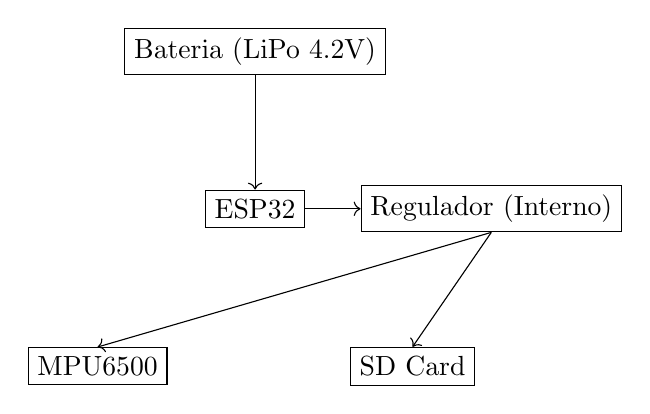
\begin{tikzpicture}
        \node[rectangle, draw] (bateria) at (0, 3) {Bateria (LiPo 4.2V)};
        \node[rectangle, draw] (esp32) at (0, 1) {ESP32};
        \node[rectangle, draw] (mpu6500) at (-2, -1) {MPU6500};
        \node[rectangle, draw] (sdcard) at (2, -1) {SD Card};
        \node[rectangle, draw] (regulador) at (3, 1) {Regulador (Interno)};

        \draw[->] (bateria.south) -- (esp32.north) node[midway, left] {};
        \draw[->] (esp32.east) -- (regulador.west) node[midway, above] {};
        \draw[->] (regulador.south) -- (mpu6500.north) node[midway, left] {};
        \draw[->] (regulador.south) -- (sdcard.north) node[midway, right] {};
    \end{tikzpicture}
    \caption{Esquemático Básico de Conexões}
    \label{fig:esquematico_basico}
\end{figure}

\paragraph{Detalhes das Conexões e Pinos}

\begin{figure}[h!]
    \centering
    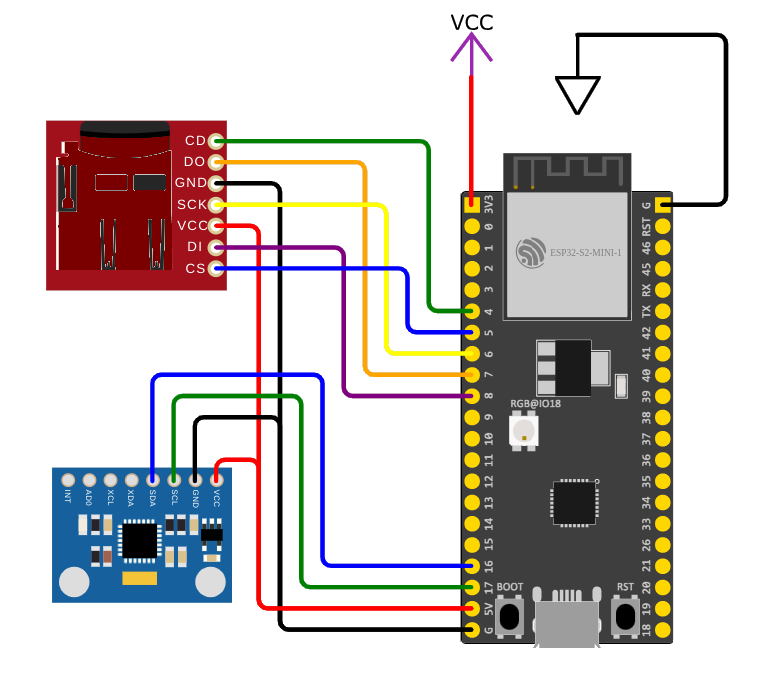
\includegraphics[width=0.8\textwidth]{figuras/eletronica-pinagem-esquematico.png}

    \caption{Esquemático de Conexões}
    \label{fig_esq_conexoes}
\end{figure}

 \textbf{Bateria LiPo (4.2V) para ESP32:}


Bateria Positivo (+) $\rightarrow$ ESP32 Vin: A entrada Vin do ESP32 aceita tensões mais altas e possui um regulador interno para fornecer a tensão de operação de 3.3V.

Bateria Negativo (-) $\rightarrow$ ESP32 GND: Todos os dispositivos devem compartilhar um terra comum para garantir o correto funcionamento do circuito.

\textbf{ESP32 para MPU-6500:}

O MPU-6500 utiliza o protocolo de comunicação I2C.

ESP32 SDA pin $\rightarrow$ MPU6500 SDA pin: O pino SDA (Serial Data) é utilizado para a transferência de dados seriais.

ESP32 SCL pin $\rightarrow$ MPU6500 SCL pin: O pino SCL (Serial Clock) é utilizado para a sincronização da transferência de dados.

ESP32 3.3V pin $\rightarrow$ MPU6500 VCC pin: O pino VCC fornece a alimentação de 3.3V necessária para o funcionamento do sensor.

ESP32 GND pin $\rightarrow$ MPU6500 GND pin: O pino GND fornece o terra para o sensor.

\textbf{ESP32 para Módulo de Cartão SD:}

O módulo de cartão SD utiliza o protocolo de comunicação SPI.

ESP32 MOSI pin $\rightarrow$ SD Card Module MOSI pin: O pino MOSI (Master Out Slave In) é utilizado para o ESP32 enviar dados para o cartão SD.

ESP32 MISO pin $\rightarrow$ SD Card Module MISO pin: O pino MISO (Master In Slave Out) é utilizado para o cartão SD enviar dados para o ESP32.

ESP32 SCK pin $\rightarrow$ SD Card Module SCK pin: O pino SCK (Serial Clock) é utilizado para a sincronização da transferência de dados.

ESP32 CS pin $\rightarrow$ SD Card Module CS pin (Chip Select): O pino CS é utilizado para selecionar o módulo de cartão SD. Este pino pode variar dependendo do módulo utilizado.

ESP32 3.3V pin $\rightarrow$ SD Card Module VCC pin: O pino VCC fornece a alimentação de 3.3V necessária para o funcionamento do módulo.

ESP32 GND pin $\rightarrow$ SD Card Module GND pin: O pino GND fornece o terra para o módulo.

\paragraph{Considerações sobre os Pinos do ESP32}

\textbf{ESP32 Vin:} A entrada Vin é projetada para aceitar tensões mais altas que 3.3V e possui um regulador de tensão interno para fornecer a tensão de operação adequada para o ESP32.

\textbf{ESP32 3.3V:} Os pinos de saída de 3.3V do ESP32 são utilizados para alimentar os sensores e o módulo de cartão SD.

\textbf{ESP32 GND:} É fundamental que todos os dispositivos no circuito compartilhem um terra comum para garantir o correto funcionamento e evitar danos aos componentes.

\textbf{ESP32 Pinos I2C:} Os pinos SDA e SCL para a comunicação I2C podem variar dependendo do modelo específico do ESP32. É comum utilizar os pinos GPIO21 (SDA) e GPIO22 (SCL), mas é essencial verificar o datasheet do seu ESP32.

\textbf{ESP32 Pinos SPI:} Os pinos MOSI, MISO e SCK para a comunicação SPI geralmente são fixos para a interface SPI principal do ESP32. No entanto, o pino CS (Chip Select) pode ser configurado em qualquer pino digital disponível.